\documentclass{article}
\usepackage{float,caption,subcaption}
\usepackage{tikz}
\usetikzlibrary{matrix,arrows}
\begin{document}

\begin{figure}[htbp]
	\centering

\begin{minipage}[t]{.4\textwidth}
\centering
\small{1. Sequentially ignorable treatment}\vspace{.25cm}
\\
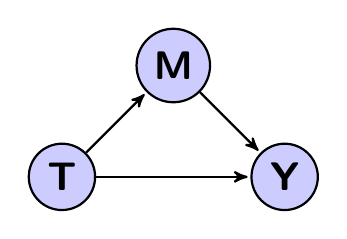
\begin{tikzpicture}[->,>=stealth',shorten >=1pt,auto,node distance=2cm,yshift=10cm,
  thick,main node/.style={circle,fill=blue!20,draw,font=\sffamily\Large\bfseries}]

  \node[main node] (1) {M};
  \node[main node] (2) [below left of=1] {T};
  \node[main node] (3) [below right of=1] {Y};


  \path[every node/.style={font=\sffamily\small}]
    (1) edge node [left] {} (3)
    (2) edge node [right] {} (1)
    (2) edge node [right] {} (3);
\end{tikzpicture}
\end{minipage}
\hfill
\begin{minipage}[t]{.45\textwidth}
\centering
\small{2. Still sequentially ignorable}\vspace{.5cm}
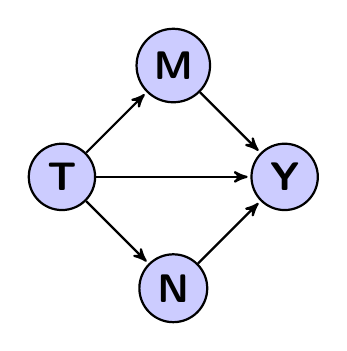
\begin{tikzpicture}[->,>=stealth',shorten >=1pt,auto,node distance=2cm,
  thick,main node/.style={circle,fill=blue!20,draw,font=\sffamily\Large\bfseries}]

  \node[main node] (1) {M};
  \node[main node] (2) [below left of=1] {T};
  \node[main node] (3) [below right of=1] {Y};
  \node[main node] (4) [below right of=2] {N};


  \path[every node/.style={font=\sffamily\small}]
    (1) edge node [left] {} (3)
    (2) edge node [right] {} (1)
    (2) edge node [right] {} (3)
    (2) edge node [left] {} (4)
    (4) edge node [left] {} (3);
\end{tikzpicture}

\end{minipage}
\vspace{1cm}

\begin{minipage}[t]{.4\textwidth}
\centering
\small{3. Not sequentially ignorable\\Pre-treatment confounder}\vspace{.25cm}
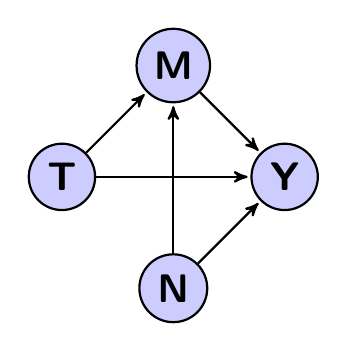
\begin{tikzpicture}[->,>=stealth',shorten >=1pt,auto,node distance=2cm,
  thick,main node/.style={circle,fill=blue!20,draw,font=\sffamily\Large\bfseries}]

  \node[main node] (1) {M};
  \node[main node] (2) [below left of=1] {T};
  \node[main node] (3) [below right of=1] {Y};
  \node[main node] (4) [below right of=2] {N};


  \path[every node/.style={font=\sffamily\small}]
    (1) edge node [left] {} (3)
    (2) edge node [right] {} (1)
    (2) edge node [right] {} (3)
    (4) edge node [left] {} (3)
    (4) edge node [left]{}(1);
\end{tikzpicture}
\end{minipage}
\hfill
\begin{minipage}[t]{.4\textwidth}
\centering
\small{4. Not sequentially ignorable\\Post-treatment confounder}\vspace{.25cm}
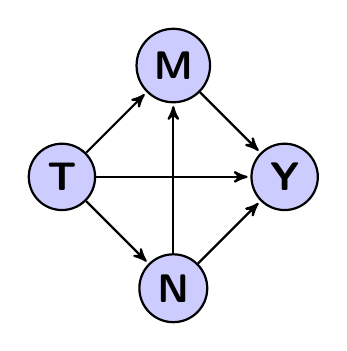
\begin{tikzpicture}[->,>=stealth',shorten >=1pt,auto,node distance=2cm,
  thick,main node/.style={circle,fill=blue!20,draw,font=\sffamily\Large\bfseries}]

  \node[main node] (1) {M};
  \node[main node] (2) [below left of=1] {T};
  \node[main node] (3) [below right of=1] {Y};
  \node[main node] (4) [below right of=2] {N};


  \path[every node/.style={font=\sffamily\small}]
    (1) edge node [left] {} (3)
    (2) edge node [right] {} (1)
    (2) edge node [right] {} (3)
    (2) edge node [left] {} (4)
    (4) edge node [left] {} (3)
    (4) edge node [left]{}(1);
\end{tikzpicture}


\end{minipage}

	\caption{Causal Mediation: In the first row, treatment is sequentially ignorable and so mediation analysis is unbiased. In the second row, mediation analysis will be biased because sequential ignorability is violated by either a pre-treatment or or post-treatment confounder. Figure adapted from Imai, Keele, and Tingley (2011) }
	\label{fig:label}
\end{figure}
\end{document}
